\subsection{Arsitektur \textit{Event-Driven} (EDA)}

Arsitektur ini tidak menggunakan PostgreSQL sama sekali. Pada dasarnya, basis data relasional terdiri atas komponen \textit{storage} dan \textit{query processor}. Pada arsitektur ini, komponen \textit{storage} diganti menggunakan Redpanda dengan berbagai topik dan \textit{query processor} diganti dengan RisingWave. Penggunaan RisingWave memungkinkan pembangunan kueri secara inkremental dari berbagai sumber data, termasuk topik Redpanda. Meskipun begitu, pendekatan ini tidak memiliki dukungan \textit{transaction} selain \textit{transaction} pada Redpanda yang berupa \textit{push log all or nothing} pada beberapa topik sekaligus. Untuk itu, Redis digunakan untuk menyimpan \textit{uncommited data} sehingga untuk mencegah \textit{double booking}.

\begin{figure}[htbp]
    \centering
    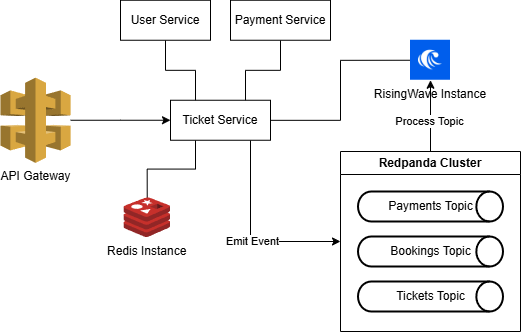
\includegraphics[width=1\textwidth]{resources/appendix/architecture-event-driven.png}
    \caption{Arsitektur EDA}
    \label{fig:solution-event-driven-architecture}
\end{figure}

\subsubsection{Pemodelan Topik dan Entitas}

Karena tidak ada basis data relasional yang digunakan dalam arsitektur ini, terdapat beberapa perubahan dalam pemodelan entitas menjadi topik. Perubahan ini adalah sebagai berikut:

\begin{enumerate}
    \item Topik Events merupakan hasil denormalisasi entitas Tickets, TicketCategory, dan Areas.
    \item Topik Seats merupakan entitas Seats. Topik ini juga menyimpan \textit{log} perubahan status \textit{seat}. Contoh: Seat-A-Available, Seat-A-Pending.
    \item Topik TicketSales merupakan hasil denormalisasi entitas TicketSale dan TicketPackage.
    \item Topik Orders merupakan hasil denormalisasi entitas Orders, OrderItem. Topik ini juga menyimpan \textit{log} perubahan status Order.
    \item Topik IssuedTickets merupakan entitas IssuedTicket.
\end{enumerate}

\subsubsection{Alur Sistem}

Berikut adalah gambaran alur sistem untuk proses pemesanan tiket dan notifikasi pembayaran.

\begin{figure}[htbp]
    \centering
    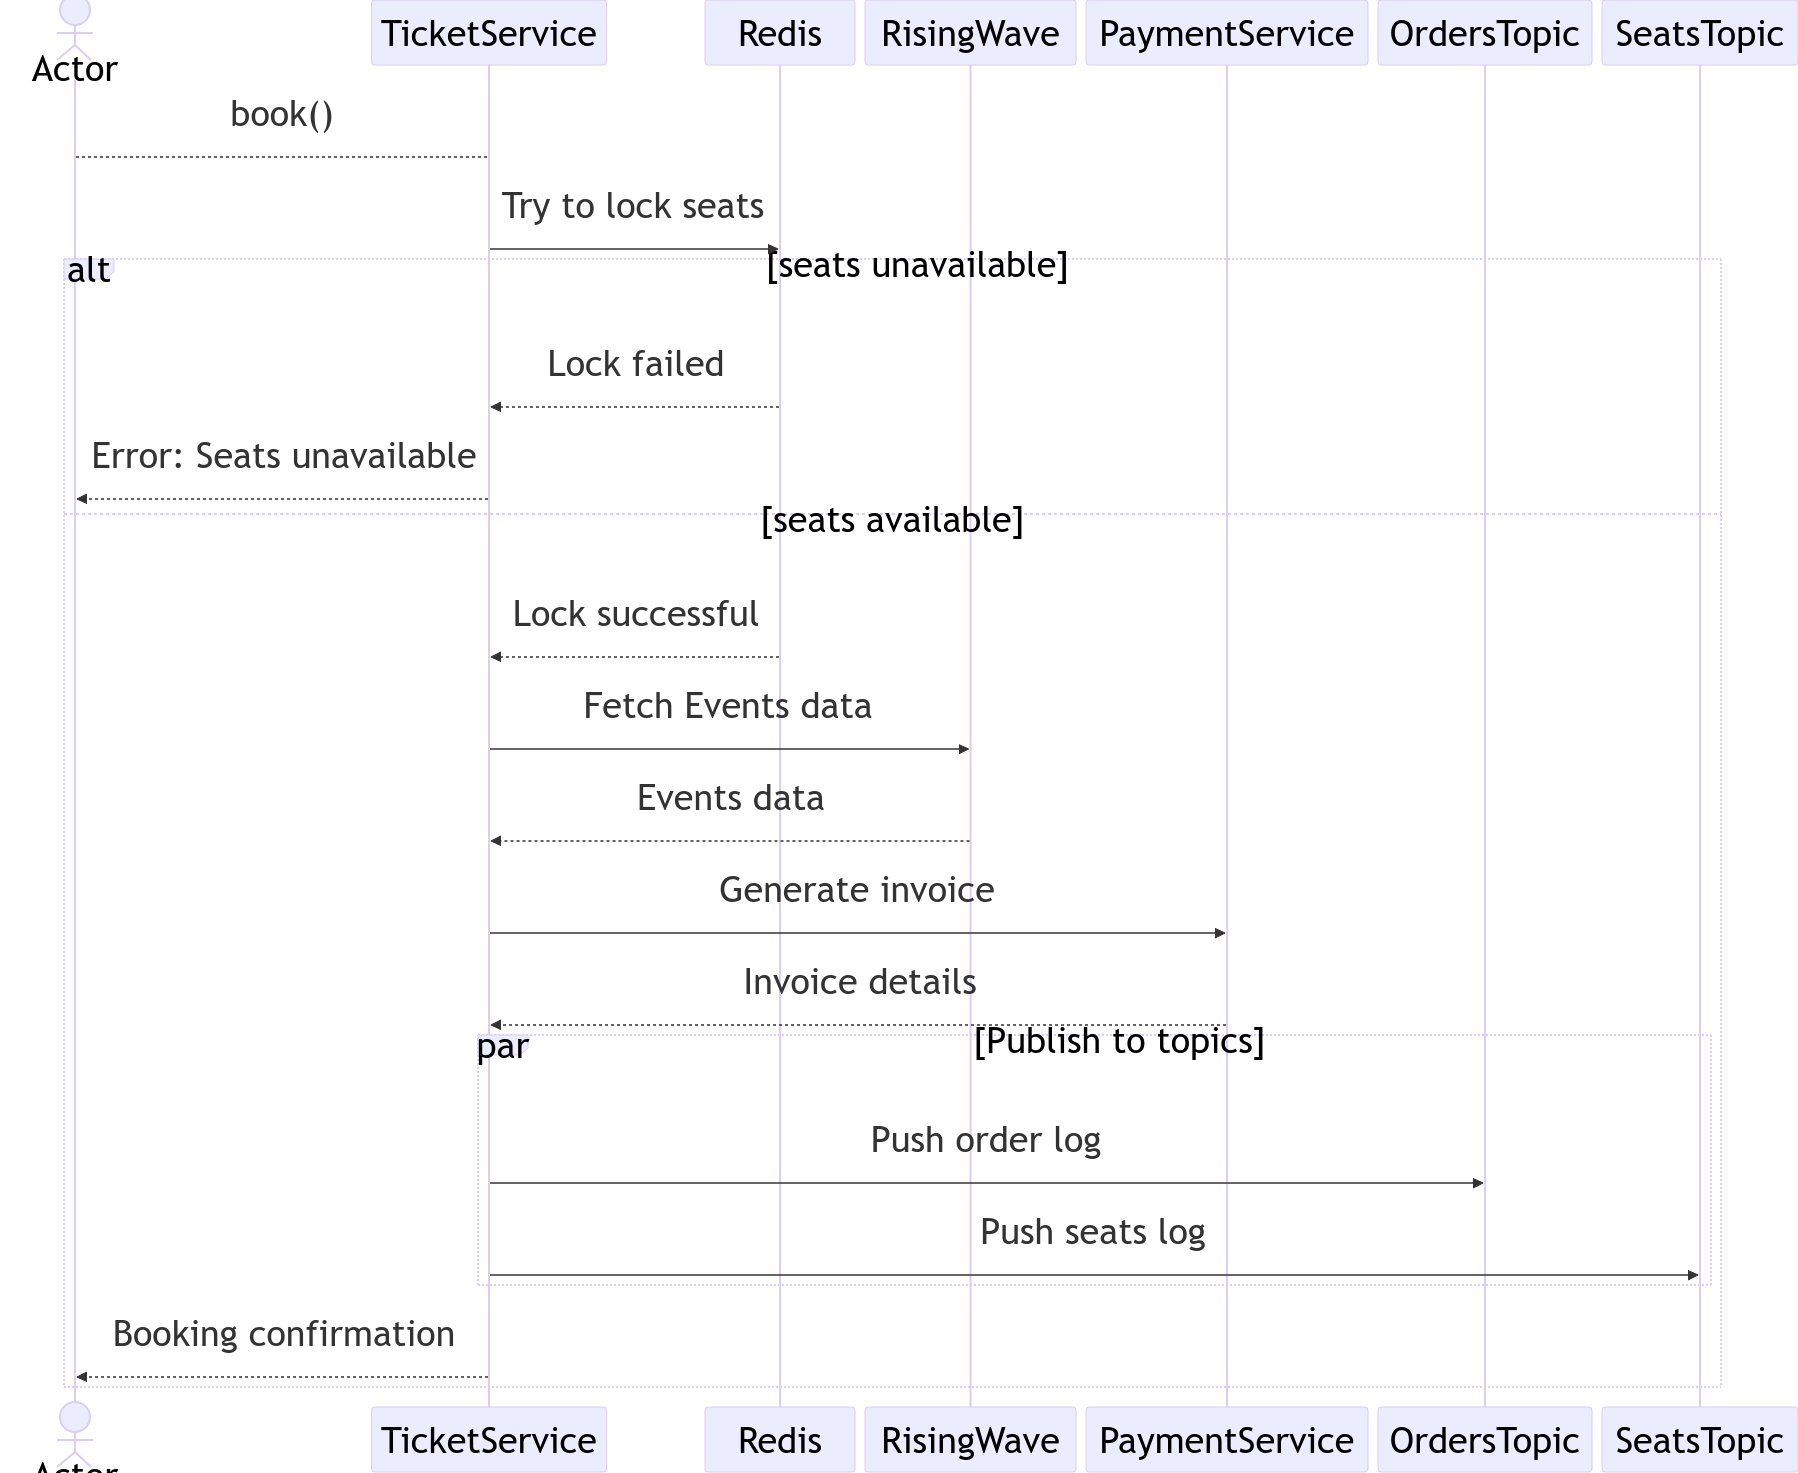
\includegraphics[width=1\textwidth]{resources/appendix/eda-book.png}
    \caption{Alur Pemesanan Tiket pada Arsitektur EDA}
    \label{fig:book-flow-eda}
\end{figure}

\begin{figure}[htbp]
    \centering
    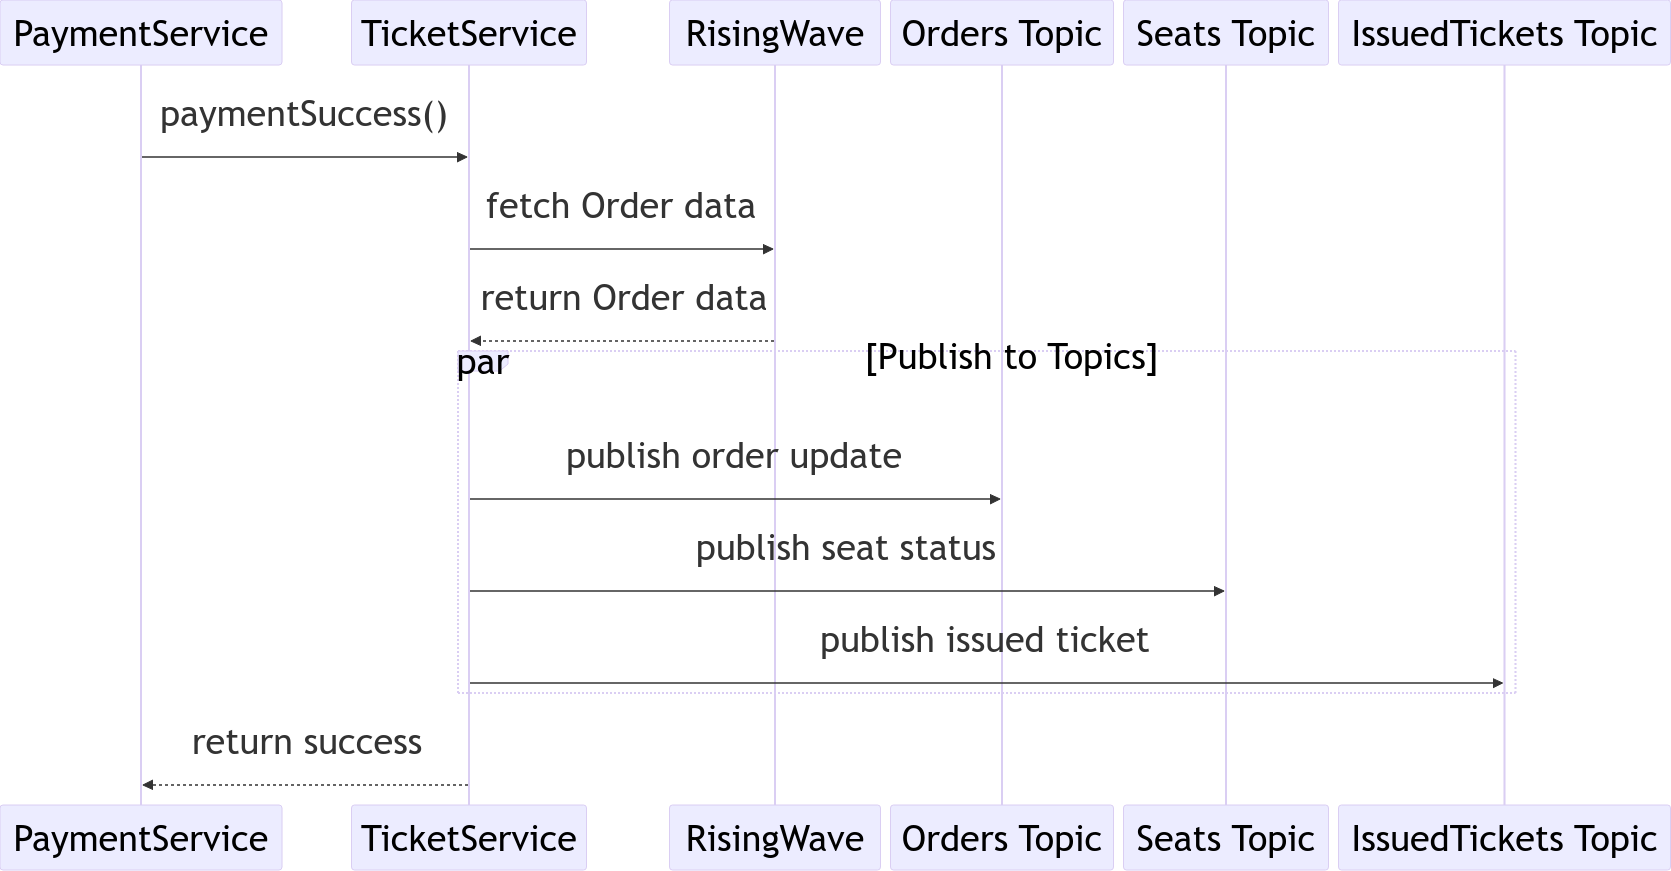
\includegraphics[width=1\textwidth]{resources/appendix/eda-verify-payment.png}
    \caption{Alur Verifikasi Pembayaran pada Arsitektur EDA}
    \label{fig:payment-verify-flow-eda}
\end{figure}

\subsubsection{Penskalaan Arsitektur EDA}

Berikut adalah strategi penskalaan untuk setiap komponen selain dengan pendekatan \textit{scale-up}:

\begin{enumerate}
    \item Layanan tiket dapat di-\textit{scale} dengan menambah jumlah \textit{instance}.
    \item Redis dapat di-\textit{scale} dengan menggunakan konfigurasi kluster, sehingga data di-\textit{shard} berdasarkan \textit{range} hash. Penskalaan ini memungkinkan peningkatan \textit{throughput} untuk operasi baca dan tulis.
    \item  RisingWave dapat di-\textit{scale} dengan meningkatkan jumlah \textit{instance}. RisingWave dapat secara otomatis mengatur penggunaan sumber daya sehingga mampu menggunakan seluruh sumber daya yang tersedia.
    \item Kluster Redpanda dapat di-\textit{scale} dengan menggunakan beberapa partisi.
\end{enumerate}

\subsubsection{Isu \textit{Persistence} Pada \textit{Uncommited Data}}

Arsitektur ini membutuhkan \textit{persistence} yang lebih kuat dibandingkan dengan arsitektur sebelumnya. Meskipun begitu, penggunaan \textit{snapshot}, AOF, dan konfigurasi \texttt{appendfsync always} dapat dianggap cukup. Perintah \texttt{appendfsync always} membuat Redis untuk selalu melakukan penulisan langsung setelah setiap perintah penulisan dijalankan. Hal ini berbeda dengan konfigurasi \textit{default} Redis yang melakukan operasi tulis setiap detik. Meskipun begitu, penggunaan konfigurasi ini menjadikan \textit{throughput} tulis Redis jauh lebih lambat. Akan tetapi, hal ini menjadi risiko yang diambil untuk menjamin \textit{safety} pada sistem ini.

\subsubsection{Aspek Lain}

\begin{enumerate}
    \item Dibandingkan dengan arsitektur sebelumnya, pendekatan seperti ini memiliki kompleksitas yang jauh lebih tinggi. Selain itu, aspek \textit{extendability} pada arsitektur ini tidak lebih baik dibandingkan dengan arsitektur sebelumnya, terutama pada penambahan fitur yang berinteraksi dengan basis data relasional.
    \item Pada saat penjualan, dapat diasumsikan entitas Events, TicketCategory, Areas, TicketSale, dan TicketPackage tidak berubah sehingga data entitas tersebut dapat di-\textit{cache}.
    \item Redis merupakan basis data yang menyimpan data di memori. \textit{Data eviction} tidak boleh terjadi ketika menggunakan Redis pada arsitektur ini, sehingga alokasi memori Redis merupakan hal yang perlu perhatian khusus.
\end{enumerate}

